\documentclass[11pt,a4paper,english]{article}
\usepackage{geometry,hologo,hyperref,babel,mdwlist,array,multicol}
\usepackage[default,osf]{sourcesanspro}
\usepackage[scaled=.95]{sourcecodepro}
\hypersetup{
    colorlinks,
    citecolor=blue,
    filecolor=blue,
    linkcolor=blue,
    urlcolor=blue
}
\newcommand*\file[1]{\href{run:#1.pdf}{#1}}

\title{\bfseries
	\Huge sourcecodepro\\
	\Large Adobe's Source Code Pro typeface for \LaTeX
}
\author{Silke Hofstra, \href{mailto:tex@slxh.nl}{tex@slxh.nl}}
\date{Documentation for sourcecodepro v2.3.\\ \today}

\begin{document}
\maketitle
\begin{multicols}{2}
This package provides the Source Code Pro font in an easy to use way. For \hologo{XeLaTeX} and \hologo{LuaLaTeX} users the original OpenType fonts are used. The entire font family is included. It can also be downloaded from \href{https://github.com/adobe/source-code-pro}{Github}.

\section{Options}
The package has the following options:
\begin{itemize*}
	\item \textbf{oldstyle, osf}:  use old style numbers.
	\item \textbf{lining, nf, lf}: use lining numbers.
	\item \textbf{black}:          \texttt{\textbackslash bfseries} is black.
	\item \textbf{semibold}:       \texttt{\textbackslash bfseries} is semibold.
	\item \textbf{bold}:           \texttt{\textbackslash bfseries} is bold.
	\item \textbf{light}:          \texttt{\textbackslash mdseries} is light.
	\item \textbf{extralight}:     \texttt{\textbackslash mdseries} is extra light.
	\item \textbf{regular}:        \texttt{\textbackslash mdseries} is regular.
	\item \textbf{scale, scaled}:  Change the scaling with a factor. For example:  \texttt{scale=.5}
	\item \textbf{default}:        Source Code Pro is set as the default font family and as the monotype family.
	\item \textbf{nottdefault}:    Source Code Pro is not set as monospaced family.
	\item \textbf{type1, t1}:      Override automatic detection and use the Type 1 fonts.
	\item \textbf{opentype, otf}:  Override automatic detection and use OpenType fonts.
\end{itemize*}
The following options are enabled by default: lining, proportional, bold and regular.

\section{Commands}
Commands for all weights are also provided for \hologo{XeTeX} and \hologo{LuaTeX} users.
\begin{itemize*}
	\item \texttt{\bfseries \textbackslash sourcecodepro}
		-- the regular and bold weights.
	\item \texttt{\bfseries \textbackslash sourcecodeprolight}
		-- the light and semibold weights.
	\item \texttt{\bfseries \textbackslash sourcecodeproextreme}
		-- the extra light and black weights.
\end{itemize*}

\section{Licence}
Adobe's Source Code Pro typeface is available under the \href{http://scripts.sil.org/OFL}{SIL Open Font License 1.1}.\\
All \LaTeX\ code is available under the \href{http://www.latex-project.org/lppl/}{\LaTeX\ project public license} v1.3 or later.

\section{Specimen}
Simple specimen can be found on page \pageref{sec:specimen}. Full specimen can be \href{http://store1.adobe.com/type/browser/pdfs/1960.pdf}{acquired from Adobe}. Please note that at the moment Source Code Pro doesn’t have italics or small-caps.

\section{OpenType}
The OpenType fonts have many features, including old style numerals (\texttt{\oldstylenums{1 6 9}})
%, ligatures (\texttt{fi fl})
and stylistic alternatives (\texttt{{\addfontfeature{Style=Alternate}a g}}).

\subsection{Features}
A complete list of available font features is available on page \pageref{sec:otfinfo}. More information on how to use font features can be found in the \href{http://mirror.ctan.org/macros/latex/contrib/fontspec/fontspec.pdf}{fontspec documentation}.

\subsection{Files}
\begin{itemize*}
	\item SourceCodePro-ExtraLight.otf
%	\item SourceCodePro-ExtraLightIt.otf
	\item SourceCodePro-Light.otf
%	\item SourceCodePro-LightIt.otf
	\item SourceCodePro-Regular.otf
%	\item SourceCodePro-RegularIt.otf
	\item SourceCodePro-Semibold.otf
%	\item SourceCodePro-SemiboldIt.otf
	\item SourceCodePro-Bold.otf
%	\item SourceCodePro-BoldIt.otf
	\item SourceCodePro-Black.otf
%	\item SourceCodePro-BlackIt.otf
\end{itemize*}

\section{Type1}
The following Type1 font families are included:
\begin{itemize*}
	\item SourceCodePro-TLF
	\item SourceCodePro-TOsF
\end{itemize*}
With series ‘el’, ‘l’, ‘m’, ‘sb’, ‘b’, ‘k’.% and shapes ‘n’, ‘i’ and ‘sc’.

\section{Version history}
\subsection*{2.3}
\begin{itemize}
	\item Fixed errors in weight implementation.
\end{itemize}

\subsection*{2.2}
\begin{itemize*}
	\item Weights are now handled with the \href{http://www.ctan.org/pkg/mweights}{mweights} package.
	\item Fixed scaling.
\end{itemize*}

\subsection*{2.1}
\begin{itemize*}
	\item Added \texttt{nottdefault} option.
	\item Fixed issue in which font was set as default sans-serif family instead of the default monospaced family.
\end{itemize*}

\subsection*{2.0}
\begin{itemize*}
	\item Merged all \texttt{.sty} files into \texttt{sourcecodepro.sty}.
	\item \texttt{default} option now sets the default font family to \texttt{Source Code Pro}, not \texttt{\textbackslash sfdefault}.
	\item \texttt{type1}, \texttt{t1}, \texttt{opentype} and \texttt{otf} option added to override automatic detection.
	\item Added \texttt{OT1} to \texttt{fontspec} options.
	\item Updated fonts to 1.017.
\end{itemize*}

\subsection*{1.02}
\begin{itemize*}
	\item Removed \texttt{proportional} and \texttt{tabular} options.
	\item Changed the order of \texttt{T1} and \texttt{LY1}.
	\item Changed \texttt{lining}/\texttt{nf} behaviour.
	\item Redefined \texttt{\textbackslash oldstylenums}.
\end{itemize*}

\section{Known issues}
\begin{itemize*}
	\item Using \texttt{\textbackslash liningnums} when the default numbers are oldstyle results in an ‘font feature does not exist’ error and no lining numbers due to lack of the ‘lnum’ font feature.
\end{itemize*}

\newpage
\end{multicols}

\section{Specimen}
At the moment Source Code Pro doesn’t have italics or small-caps.
\label{sec:specimen}
\subsection{OpenType}
\begin{figure}[ht]
	\centering
	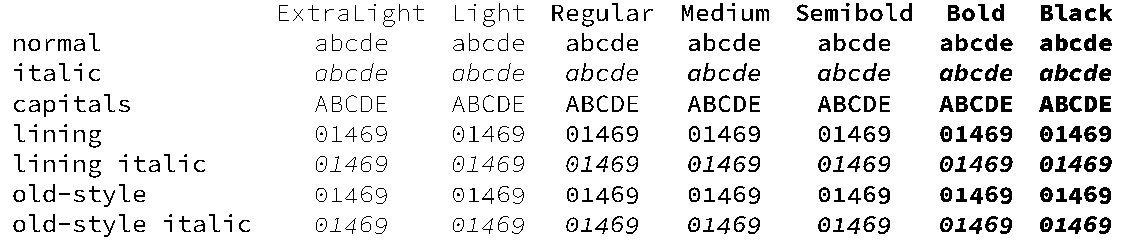
\includegraphics{sourcecodepro-otf-specimen}
\end{figure}
This table can also be found in \file{sourcecodepro-otf-specimen}.

\subsection{Type1}
\begin{figure}[ht]
	\centering
	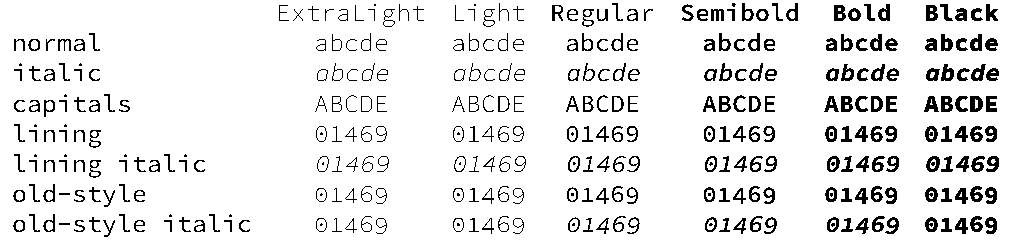
\includegraphics{sourcecodepro-type1-specimen}
\end{figure}
This table can also be found in \file{sourcecodepro-type1-specimen}.

\newpage
\section{Opentype features}
\label{sec:otfinfo}

\begin{figure}[ht]
	\centering
	\begin{tabular}{>{\ttfamily}l l}
		aalt & Access All Alternates \\
		case & Case-Sensitive Forms \\
		ccmp & Glyph Composition/Decomposition \\
		dnom & Denominators \\
		frac & Fractions \\
		mark & Mark Positioning \\
		mkmk & Mark to Mark Positioning \\
		numr & Numerators \\
		onum & Oldstyle Figures \\
		ordn & Ordinals \\
		salt & Stylistic Alternates \\
		sinf & Scientific Inferiors \\
		size & Optical Size \\
%		ss01 & Stylistic Set 1 - alternate l \\
		ss02 & Stylistic Set 2 - alternate a \\
		ss03 & Stylistic Set 3 - alternate g \\
%		ss04 & Stylistic Set 4 - alternate I \\
		subs & Subscript \\
		sups & Superscript	
	\end{tabular}
\end{figure}
\textit{(list generated with otfinfo)}

\end{document}

